\documentclass[notheorems, serif, table, compress]{beamer}  %dvipdfm选项是关键, 否则编译统统通不过
%%------------------------常用宏包------------------------
%%注意,  beamer 会默认使用下列宏包: amsthm,  graphicx,  hyperref,  color,  xcolor,  等等
\usepackage{fontspec, xunicode, xltxtra}  % for XeTeX
\usepackage{verbatim}
\usepackage{mathabx}
\usepackage{latexsym}
\usepackage{amsfonts, amssymb}
\usepackage{styles/iplouclistings}
\usepackage{fancybox}
\usepackage{colortbl}
\usepackage{tcolorbox}
%\usepackage[T1]{fontenc}
%\usepackage{bookman}
\usepackage{subfigure}
\usepackage{hyperref}
\usepackage{listings}
\usepackage{animate}
\usepackage[absolute, overlay]{textpos}
\usepackage{graphicx}
\usepackage{tikz}
\usepackage[americaninductors, europeanresistors]{circuitikz}
\usepackage{tikz}
\usepackage{fancybox}     %% 定义zhushadow时用到
\usepackage{pifont} %ding用到
\newsavebox{\mysaveboxOne}  %%为了在only中使用lstlisting
\newsavebox{\mysaveboxTwo}
\newsavebox{\mysaveboxThree}
\newsavebox{\mysaveboxFour}
\newsavebox{\mysaveboxFive}
\newsavebox{\mysaveboxSix}
\newsavebox{\mysaveboxSeven}
\newcommand\zhushadow[2][purple]{\hskip5pt\shadowbox{\color{#1}\small\kai #2\vspace{3mm}}}

%%------------------------ThemeColorFont------------------------
%% Presentation Themes
% \usetheme[<options>]{<name list>}
%\usetheme{Madrid}
\usetheme{Berkeley}
%% Inner Themes双精度计算
% \useinnertheme[<options>]{<name>}
%% Outer Themes
% \useoutertheme[<options>]{<name>}
%\useoutertheme{miniframes} 
%% Color Themes 
%\usecolortheme[<options>]{<name list>}
%% Font Themes
\usefonttheme{serif}
\setbeamertemplate{background canvas}[vertical shading][bottom=white, top=structure.fg!7] %%背景色,  上25%的蓝,  过渡到下白.
\setbeamertemplate{theorems}[numbered]
\setbeamertemplate{navigation symbols}{}   %% 去掉页面下方默认的导航条.
\usepackage{styles/zhfontcfg}
%\setsansfont[Mapping=tex-text]{文泉驿正黑}  %% 需要fontspec宏包
     %如果装了Adobe Acrobat, 可在font.conf中配置Adobe字体的路径以使用其中文字体
     %也可直接使用系统中的中文字体如SimSun, SimHei, 微软雅黑 等
     %原来beamer用的字体是sans family;注意Mapping的大小写, 不能写错
     %设置字体时也可以直接用字体名,以下三种方式等同:
     %\setromanfont[BoldFont={黑体}]{宋体}
     %\setromanfont[BoldFont={SimHei}]{SimSun}
     %\setromanfont[BoldFont={"[simhei.ttf]"}]{"[simsun.ttc]"}
%%------------------------MISC------------------------
\graphicspath{{figures/}}         %% 图片路径. 本文的图片都放在这个文件夹里了.
%%------------------------listing------------------------
%\lstset{language=[LaTeX]TeX, Python}
%%------------------------正文------------------------
\begin{document}
\XeTeXlinebreaklocale "zh"         % 表示用中文的断行
\XeTeXlinebreakskip = 0pt plus 1pt % 多一点调整的空间
%%----------------------------------------------------------
%% This is only inserted into the PDF information catalog. Can be left
%% out.
%%%
%% Delete this,  if you do not want the table of contents to pop up at
%% the beginning of each subsection:
%\AtBeginSection[]{                              % 在每个Section前都会加入的Frame
%  \frame<handout:0>{
%    \frametitle{Contents}\small
%    \tableofcontents[current, currentsubsection]
%  }
%}
%
%\AtBeginSubsection[]                            % 在每个子段落之前
%{
%  \frame<handout:0>                             % handout:0 表示只在手稿中出现
%  {
%    \frametitle{Contents}\small
%    \tableofcontents[current, currentsubsection] % 显示在目录中加亮的当前章节
%  }
%}

\setbeamertemplate{caption}{\raggedright\insertcaption\par}

%%----------------------------------------------------------
\logo{
\includegraphics[scale=0.13]{ouclogo.png}}
\title{Digital Image Processing Learning}
%\subtitle{Bottom-Up Saliency Detection Model Based on Human Visual Sensitivity and Amplitude Spectrum}
\subtitle{The third section}
\author[]{\textcolor{olive}{常琳}}
\institute[CVBIOUC]
{
\small\textcolor{violet}{CVBIOUC\\
%Ocean University of China\\
\url{http://vision.ouc.edu.cn/~zhenghaiyong}}
}
%\date[]{}
%\titlegraphic{
%\includegraphics[height=1.0cm]{ouc-logo.jpg}}
\frame{ \titlepage }
%%----------------------------------------------------------
%\section*{Contents}
\frame{\frametitle{Contents}\tableofcontents}
%%----------------------------------------------------------
\def\hilite<#1>{\temporal<#1>{\color{blue!15}}{\color{black}}{\color{black}}}
\newcommand{\shadow}[2][purple]{\hskip5pt\shadowbox{\color{#1}\small \kai #2\vspace{3mm}}}
\newcommand{\colorrbox}[2][purple]{\doublebox{\color{#1}\small \kai#2}}

%============================================================================

\section{Intensity Transformations }

%==========================================================================


\begin{frame}[fragile]
\frametitle{Purpose}

We want to:

\begin{description}
\item [Contrast manipulation and image thresholding]Intensity Transformation %对比度和阈值处理为目的 :灰度变换
\item [Performing operations]Spatial filtering %改善性能: 空间滤波
\end{description}
\end{frame}
%=======================================================================
\subsection{Some Basic Intensity Transformation Functions}%一些基本灰度变换函数
\begin{frame}
\frametitle{Some Basic Intensity Transformation Functions}
 

\begin{description}
\item [linear] Image Negatives, $s=L-1-r$.  %图像反转
\end{description}
Enhance white or gray detail embedded in dark regions of an image.%增强嵌入在一幅图像暗区域中的白色或灰色细节



 \begin{figure}[!ht]
  \begin{minipage}[t]{0.4\textwidth}	
  \centering
  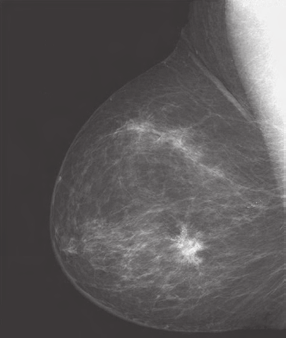
\includegraphics[width=1.5in]{fanzhuan.png}
  \caption{Figure1(a), Original picture}
  \end{minipage}
  \begin{minipage}[t]{0.4\textwidth}
  \centering
  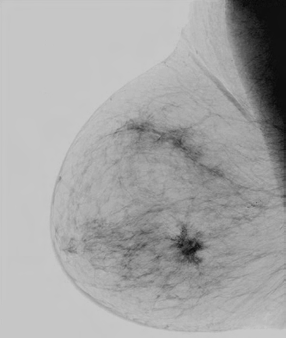
\includegraphics[width=1.5in]{fanzhuanout.png}
  \caption{Figure1(b), Using the negative transformation}
  \end{minipage}
  \end{figure} 

\end{frame}

\begin{frame}

\frametitle{Some Basic Intensity Transformation Functions}
    
\begin{description}
\item [Logarithmic]Log transformation, $s = clog(1 + r)$.

\end{description}
 We use this type to expand the values of dark pixels in an image while compressing the higher-level values.
%我们用这种变换扩展图像中暗像素的值, 同时压缩更高灰度级的值
\end{frame}



\begin{frame}
\frametitle{Some Basic Intensity Transformation Functions}
    
\begin{description}
\item [Power-law] Power-Law(Gamma)transformstions, $s=cr^\gamma$.
\end{description}

  Depend on $\gamma$.

\begin{figure}[!ht]
  \begin{minipage}[t]{0.4\textwidth}	
  \centering
  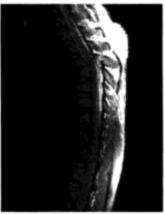
\includegraphics[width=1.1in]{spine.png}
  \caption{Figure2(a), Original picture}
  \end{minipage}
  \begin{minipage}[t]{0.4\textwidth}
  \centering
  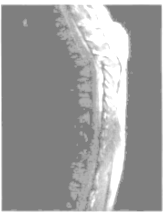
\includegraphics[width=1.1in]{spineout.png}
  \caption{Figure2(b), $\gamma=0.5$}
  \end{minipage}
  \end{figure} 

\end{frame}



\begin{frame}
\frametitle{Some Basic Intensity Transformation Functions}
    
\begin{description}
 \item[Piecewise-Linear Transformationn Functions]

Advantage:can be arbitrarily complex.

Disadvantage :their specification requires considerably more user input.
\end{description}
%分段线性变换函数]优点:形式可以是任意复杂的。\quad 缺点:技术说明要求用户输入

\end{frame}
%=====================================================================



\subsection{Histogram Processing}%直方图处理
 \begin{frame}
\frametitle{Histogram Processing}
 For image enhancement.
    
Normallize a histogram:$p(r_{k})=n_{k}/MN$, for $k=0, 1, .....L-1, p_{k}$ is an estimate of the probability of occurrence of intensity level $r_{k}$ in an image.The sum of all components of a normalized histogram is equal to 1.

%归一化直方图:$p(r_{k})=n_{k}/MN$, 其中$k=0, 1, .....L-1, p_{k}$是灰度级$r_{k}$在图像中出现的概率的一个估计。归一化直方图的所有分量之和应等于1。
    
 \end{frame}



\begin{frame}
\frametitle{Histogram Equalization}%直方图均衡
  Spread the histogram of the input image so that the intensity levels of the equalized image span a wider range of the intensity scale.The net result is contrast enhancement.
%展开输入图像直方图的趋势,均衡后的图像的灰度级跨越更宽灰度级范围,最终结果是增强了对比度。

 The results are predictable and method is simple to implement.%结果可预知,方法简单

Equations:
   \begin{equation}    \label{3.8} %????
    p_{r}(r_{k})= \frac{n_{k}}{MN}, k=0, 1, 2\ldots, L-1
   \end{equation}

   \begin{equation} \label {3.9}
     s_{k}=T(r_{k})=(L-1)\sum_{j=0}^{k}p_{r}(r_{j})=\frac{(L-1)}{MN} \sum_    {j=0}^{k}{n_{j}}, k=0, 1-2\ldots, L-1
   \end{equation}
 \end{frame}

\begin{frame}
\frametitle{Histogram Equalization}%直方图均衡
 \begin{figure}
        \begin{minipage}[t]{0.4\linewidth}
        \centering
        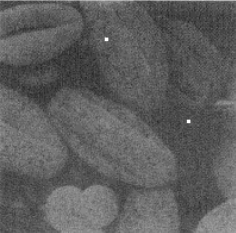
\includegraphics[width=0.6\linewidth]{huafen.png} 
        \caption{Figure3(a), Original picture}
        \end{minipage}
        \begin{minipage}[t]{0.4\linewidth}
        \centering
        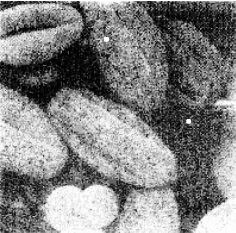
\includegraphics[width=0.6\linewidth]{huafeneq.png} 
          \caption{Figure3(b), Equalization}
        \end{minipage}
    \end{figure}

\begin{figure}
        \begin{minipage}[t]{0.4\linewidth}
        \centering
        
\includegraphics[width=0.6\linewidth]{huafenzhifang.png} 
        \caption{Figure3(c), Original histogram}
        \end{minipage}
        \begin{minipage}[t]{0.4\linewidth}
        \centering
        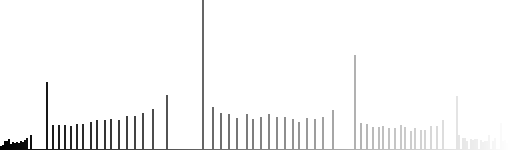
\includegraphics[width=0.6\linewidth]{huafeneqzhifang.png} 
          \caption{Figure3(d), Histogram after equalizing}
        \end{minipage}
    \end{figure}
\end{frame}




\begin{frame}
\frametitle{Histogram matching} %直方图匹配
    
The method used to generate a processed image that has a specified histogram.

%直方图匹配:用于产生处理后有特殊直方图的方法。

Major equations:
 \begin{equation} \label {3.13}
s_{k}=T(r_{k})=(L-1)\sum_{j=0}^{k}p_{r}(r_{j})=\frac{(L-1)}{MN}\sum_{j=0}^{k}{n_{j}}, k=0, 1, 2\ldots, L-1
\end{equation}
 
  \begin{equation} \label {3.14}
G(z_{q})=(L-1)\sum_{i=0}^{q}p_{z}(z_{i})
\end{equation}
\end{frame}

\begin{frame}
\frametitle{Histogram matching}
\begin{equation} \label {3.15}
G(z_{q})=s_{k}
\end{equation}
$p_z(z_{i})$ is the $i$th value of the specified histogram.

\begin{equation} \label {3.16}
z_{q}=G^{-1}(s_{k})
\end{equation}
\end{frame}



\subsubsection{Local Histogram Processing}%局部直方图处理
\begin{frame}
\frametitle{Local Histogram Processing}
Enhance details over small areas in an image.%增强图像中小区域的细节

\end{frame}
%=======================================================================
\begin{frame}
\frametitle{Using Histogram Statistics for Image Enhancement}%在图像增强中使用直方图统计

 
 The  mean and variance are used as the basis for making changes.

%均值和方差是图像特征进行改变的基础。

 
\end{frame}
%========================================================================
\section{Spatial Filtering}%空间滤波
\subsection{Fundamentals of Spatial Filtering}
\begin{frame}
\frametitle{Fundamentals of Spatial Filtering}
 Spatial filters can be used also for nonlinear filtering, something we cannot do in the frequency domain.
%空间滤波可用于非线性滤波,在频率域中做不到。
 Linear spatial filtering of an image of size $M*N$ with a filter of size $m*n$ is given by the expression:

%使用大小为$m*n$ 的滤波器对大小为$M*N$的图像进行线性空间滤波,可由下式表示:

\begin{equation} \label {3.13}
g(x, y)=\sum_{s=-a}^{a}\sum_{t=-b}^{b}w(s, t)f(x+s, y+t)
\end{equation}
 \end{frame}

\subsection{Smoothing Spatial Filters}%平滑空间滤波器
\begin{frame}
\frametitle{Smoothing Linear Filters}%平滑线性滤波器

Smoothing filters are used for blurring and for noise reduction.
%平滑滤波器用于模糊处理和降低噪声。

The output(response) of a smoothing, linear spatial filter  is  the average of the pixels contained in the neighborhood of the filter mask.
 
Sometimes are called averaging filters.Refer to a lowpass filters.
%平滑线性空间滤波器的输出(响应)是包含在滤波器模板邻域内的像素的简单平均值。这些滤波器有时也称为均值滤波器。归入低通滤波器。

A major use of averaging filters is in the reduction of ”irrelevant” detail in an image.
%均值滤波器主要应用是去除图像中的不相关细节
 \end{frame}



\begin{frame}
\frametitle{Order-Statistic(Nonlinear) Filters}%统计排序(非线性)滤波器
 The best-known filter is the medium filter.
 %最有名的是中值滤波器。
 
Median Filters are particularly effective in the presence of impulse noise, also called salt-and pepper noise.

%中值滤波器对处理脉冲噪声非常有效,也称椒盐噪声。
 \end{frame}



\begin{frame}
\frametitle{Dealing with noise}
  \begin{figure}
            \begin{minipage}[t]{0.3\linewidth}
            \centering
            
            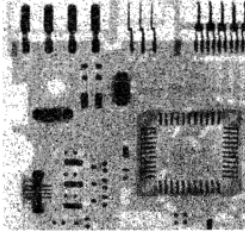
\includegraphics[width=1\linewidth]{medium.png} 
\caption{Original image}
            \end{minipage}
            \begin{minipage}[t]{0.3\linewidth}
            \centering
            
            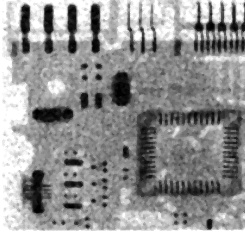
\includegraphics[width=1\linewidth]{medout.jpg} 
            
\caption{Median filter}
\end{minipage}
            \begin{minipage}[t]{0.3\linewidth}
            \centering
            
            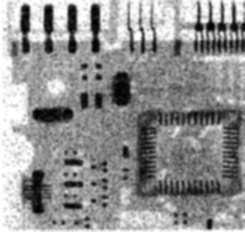
\includegraphics[width=1\linewidth]{aveout.jpg} 
            \caption{Average filter}
\end{minipage}
        \end{figure}
 \end{frame}

\subsection{Sharpening Spatial Filters}
\begin{frame}
\frametitle{Sharpening Spatial Filters}% 锐化空间滤波器
 Highlight transitions in intensity.

%锐化处理的主要目的是突出灰度的过渡部分。

Using the the Laplacian for Image Sharpening 
%使用二阶微分的拉普拉斯算子进行图像锐化——

\begin{equation} \label{3.30}
 \frac{\partial^{2}f}{\partial x^{2}}=f(x+1)+f(x-1)-2f(x)
\end{equation}

\begin{equation} \label{3.31}
 \frac{\partial^{2}f}{\partial y^{2}}=f(y+1)+f(y-1)-2f(y)
\end{equation}

\begin{equation} \label{3.32}
\bigtriangledown^{2}f= f(x+1, y)+f(x-1, y)+f(x, y+1)+f(x, y-1)-4f(x, y)
\end{equation}
\begin{equation} \label{3.33}
g(x, y)=f(x, y)+c[\bigtriangledown^{2}f(x, y)]
\end{equation}
 \end{frame}


\begin{frame}
\frametitle{Sharpening Spatial Filters}
 The Laplacian is used for highlights intensity discontinuities in an image.This will tend to produce images that have grayish edge lines and other discontinuities, all superimposed on a dark, featureless background.
Background features can be "recovered" while still preserving the sharpening effect of the Laplacian simply by adding the Laplacian image to the original.

%拉普拉斯算子算子的应用强调的是图像中灰度的突变。这将产生把浅灰色边线和突变点叠加到暗色背景中的图像。将源图像和拉普拉斯图像叠加在一起的简单方法,可以恢复原背景特性并保持拉普拉斯锐化处理的效果。

\end{frame}



\begin{frame}
\frametitle{Unsharp Masking and Highboost Filtering}% 非锐化掩蔽和高提升滤波
 A process that has been used to sharpen images consists of subtracting an unsharp(smoothed) version of an image from the original image.Then add the difference.
%图像锐化处理过程是从原图像中减去一幅非锐化(平滑过的),再用原图加上差值。

\end{frame}
\subsection{Combining Spatial Enhancement Methods}%混合空间增强法
\begin{frame}
\frametitle{Combining Spatial Enhancement Methods}
 Combine several approaches.
 \end{frame}
%============================================================================
\section{Problems for myself}

 汇报:
\begin{enumerate}
\item 对于内容的理解。
\item 形式的展示,觉得需要的内容就放上,但可以快速讲过,最好是加上个人的理解与体会而不是照搬书本。汇报如何吸引人?
\item 发现问题,寻找解决问题的上路,方法,发现问题后深入思考下去。
\end{enumerate}

平时:
\begin{enumerate}
\item 把不会的表达出来。
\item 学习内容上的深度交流。
\item 报告形式上多学习,多问。
\end{enumerate}


%===============================================================================


\end{document}
